\documentclass[]{ximera}
%handout:  for handout version with no solutions or instructor notes
%handout,instructornotes:  for instructor version with just problems and notes, no solutions
%noinstructornotes:  shows only problem and solutions

%% handout
%% space
%% newpage
%% numbers
%% nooutcomes

%I added the commands here so that I would't have to keep looking them up
%\newcommand{\RR}{\mathbb R}
%\renewcommand{\d}{\,d}
%\newcommand{\dd}[2][]{\frac{d #1}{d #2}}
%\renewcommand{\l}{\ell}
%\newcommand{\ddx}{\frac{d}{dx}}
%\everymath{\displaystyle}
%\newcommand{\dfn}{\textbf}
%\newcommand{\eval}[1]{\bigg[ #1 \bigg]}

%\begin{image}
%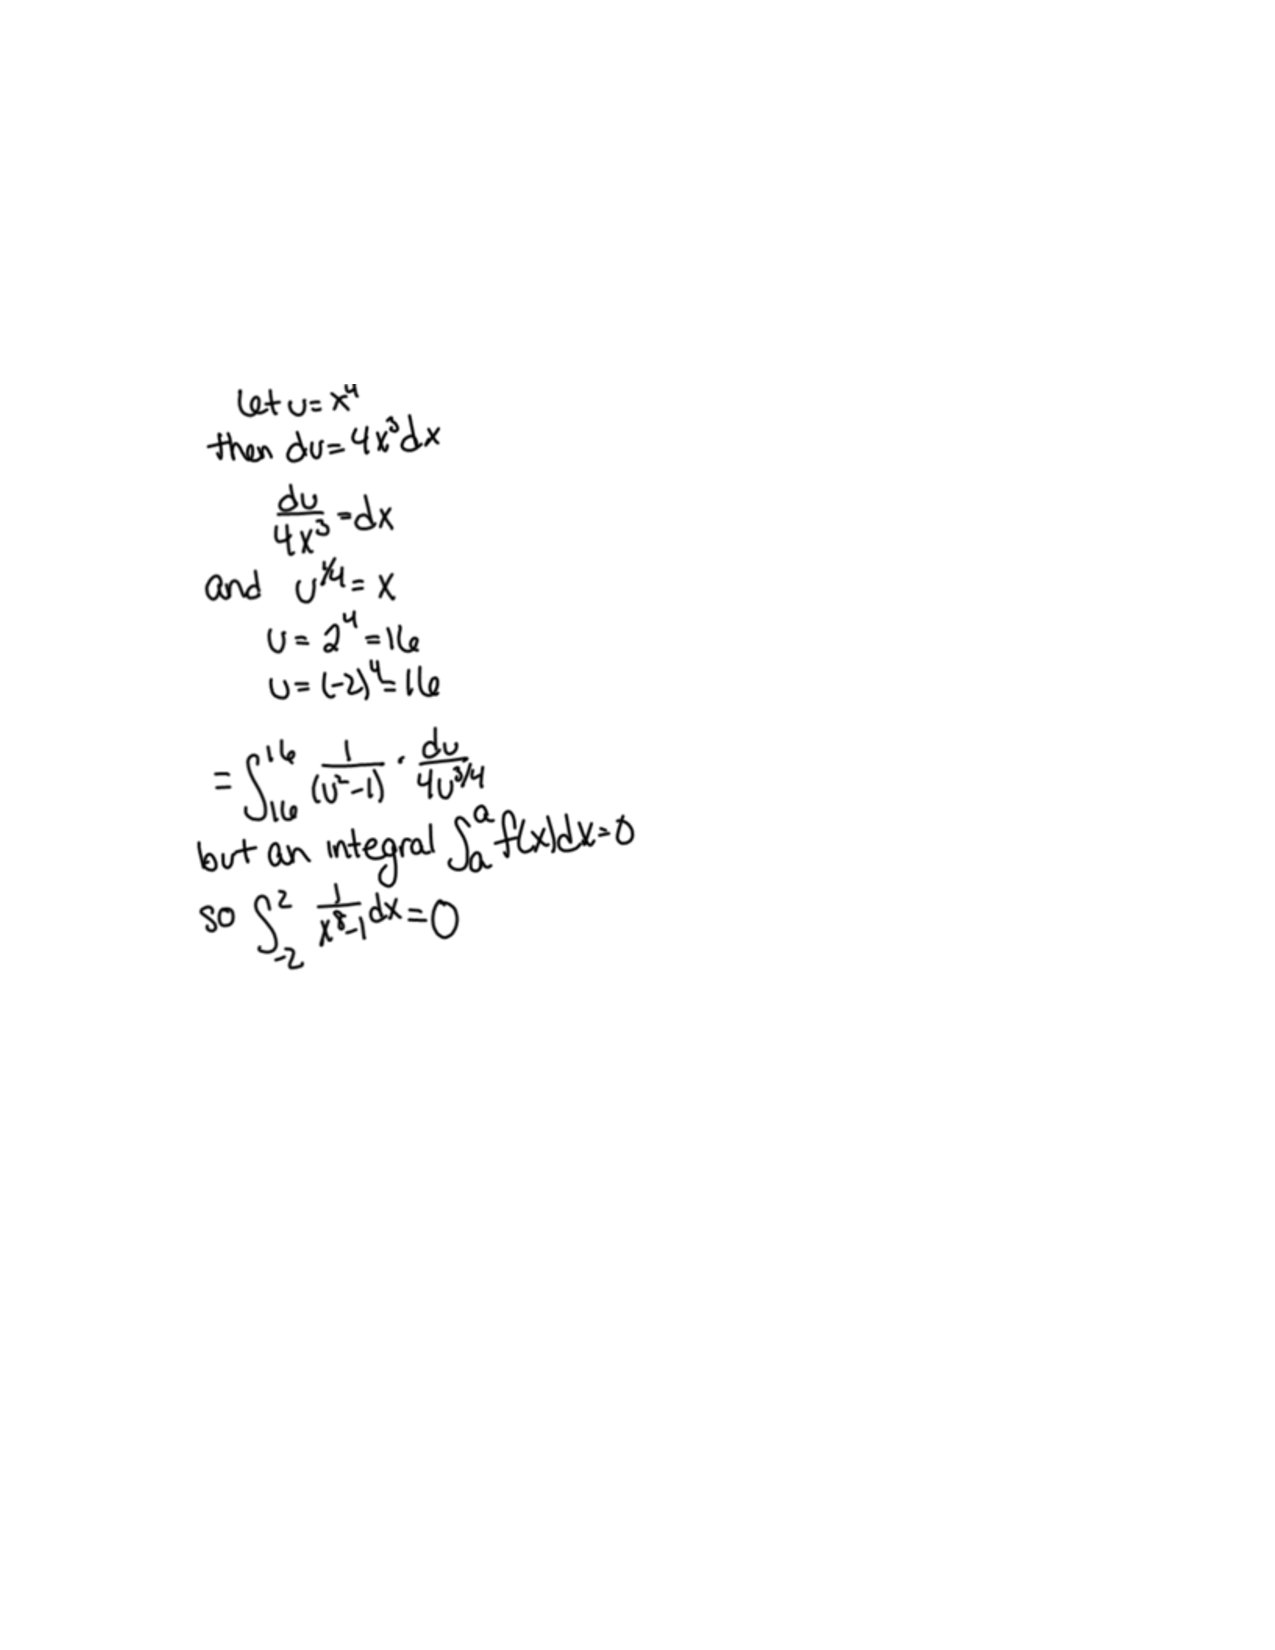
\includegraphics[trim= 170 420 250 180]{Figure1.pdf}
%\end{image}

%add a ``.'' below when used in a specific directory.
\newcommand{\RR}{\mathbb R}
\renewcommand{\d}{\,d}
\newcommand{\dd}[2][]{\frac{d #1}{d #2}}
\renewcommand{\l}{\ell}
\newcommand{\ddx}{\frac{d}{dx}}
\newcommand{\dfn}{\textbf}
\newcommand{\eval}[1]{\bigg[ #1 \bigg]}

\usepackage{multicol}

\renewenvironment{freeResponse}{
\ifhandout\setbox0\vbox\bgroup\else
\begin{trivlist}\item[\hskip \labelsep\bfseries Solution:\hspace{2ex}]
\fi}
{\ifhandout\egroup\else
\end{trivlist}
\fi} %% we can turn off input when making a master document

\title{Vectors in the plane}  

\begin{document}
\begin{abstract}		\end{abstract}
\maketitle



\begin{comment}
\section{Warm up:}

	\begin{freeResponse}
	
	\end{freeResponse}
	
\begin{instructorNotes}

\end{instructorNotes}
\end{comment}







\section{Group work:}



%problem 1
\begin{problem}
Assume that $\vec{u} = \frac{1}{2} \hat{\imath} + \frac{\sqrt{3}}{2} \hat{\jmath}$ and $\vec{v} = \frac{\sqrt{3}}{2} \hat{\imath} - \frac{1}{2} \hat{\jmath}$.
	\begin{enumerate}
	\item  Show that $\vec{u}$ and $\vec{v}$ are perpendicular unit vectors.
	\item  Write $\hat{\imath}$ as $a_1 \vec{u} + b_1 \vec{v}$ for some real numbers $a_1$ and $b_1$.  
	\item  Write $\hat{\jmath}$ as $a_2 \vec{u} + b_2 \vec{v}$ for some real numbers $a_2$ and $b_2$. 
	\end{enumerate}
	
	\begin{freeResponse}
	\begin{enumerate}
	\item  First, to show that both vectors are unit vectors, we take their norms and show that they are equal to one.
		\begin{align*}
		&\| \vec{u} \| = \sqrt{ \left( \frac{1}{2} \right)^2 + \left( \frac{\sqrt{3}}{2} \right)^2} = \sqrt{ \frac{1}{4} + \frac{3}{4}} = 1  \\
		&\| \vec{v} \| = \sqrt{ \left( \frac{\sqrt{3}}{2} \right)^2 + \left( - \frac{1}{2} \right)^2} = \sqrt{\frac{3}{4}+\frac{1}{4}} = 1.
		\end{align*}
	
	Now, to show that the two vectors are perpendicular, we take their dot product and show that it is equal to $0$.
		\begin{align*}
		\vec{u} \cdot \vec{v}
		&= \left\langle \frac{1}{2}, \frac{\sqrt{3}}{2} \right\rangle \cdot \left\langle \frac{\sqrt{3}}{2}, - \frac{1}{2} \right\rangle  \\
		&= \left( \frac{1}{2} \right) \left( \frac{\sqrt{3}}{2} \right) + \left( \frac{\sqrt{3}}{2} \right) \left( - \frac{1}{2} \right)  \\
		&= \frac{\sqrt{3}}{4} - \frac{\sqrt{3}}{4} = 0.
		\end{align*}
	
	
	
	\item  
		\begin{align}
		\hat{\imath} &= a_1 \vec{u} + b_1 \vec{v}  \nonumber \\
		&= a_1 \left( \frac{1}{2} \hat{\imath} + \frac{\sqrt{3}}{2} \hat{\jmath} \right) + b_1 \left( \frac{\sqrt{3}}{2} \hat{\imath} - \frac{1}{2} \hat{\jmath} \right)  \nonumber \\
		&= \left( \frac{1}{2} a_1 + \frac{\sqrt{3}}{2} b_1 \right) \hat{\imath} + \left( \frac{\sqrt{3}}{2} a_1 - \frac{1}{2} b_1 \right) \hat{\jmath}.  \label{equation 1}
		\end{align}
	Therefore, we must have that
		\[
		\frac{1}{2} a_1 + \frac{\sqrt{3}}{2} b_1 = 1 	\qquad	\text{and} 	\qquad	\frac{\sqrt{3}}{2} a_1 - \frac{1}{2} b_1 = 0.
		\]
	Solving the right-hand equation for $b_1$ we have that
		\[
		b_1 = \sqrt{3} a_1.
		\]
	Plugging this into the left-hand equation gives
		\begin{align*}
		&1 = \frac{1}{2} a_1 + \frac{\sqrt{3}}{2} \cdot \sqrt{3} a_1  \\
		\Longrightarrow \qquad &1 = \frac{1}{2} a_1 + \frac{3}{2} a_1 = 2 a_1  \\
		\Longrightarrow \qquad &a_1 = \frac{1}{2}.
		\end{align*}
	So $b_1 = \frac{\sqrt{3}}{2}$, and therefore
		\[
		\boxed{\hat{\imath} = \frac{1}{2} \vec{u} + \frac{\sqrt{3}}{2} \vec{v}}.
		\]
	
	
	
	\item  In the same manner as in equation \eqref{equation 1} we have that
		\[
		\hat{\jmath} = \left( \frac{1}{2} a_2 + \frac{\sqrt{3}}{2} b_2 \right) \hat{\imath} + \left( \frac{\sqrt{3}}{2} a_2 - \frac{1}{2} b_2 \right) \hat{\jmath}
		\]
	and so
		\[
		\frac{1}{2} a_2 + \frac{\sqrt{3}}{2} b_2 = 0 	\qquad	\text{and} 	\qquad	\frac{\sqrt{3}}{2} a_2 - \frac{1}{2} b_2 = 1.
		\]
	Now, solving the left-hand equation for $a_2$ gives
		\[
		a_2 = - \sqrt{3} b_2.
		\]
	Then plugging into the right-hand equation yields
		\begin{align*}
		&1 = \frac{\sqrt{3}}{2} \cdot (- \sqrt{3} b_2 ) - \frac{1}{2} b_2  \\
		\Longrightarrow \qquad &1 = - \frac{3}{2} b_2 - \frac{1}{2} b_2 = -2 b_2  \\
		\Longrightarrow \qquad &b_2 = - \frac{1}{2}.
		\end{align*}
	So $a_2 = \frac{\sqrt{3}}{2}$, and therefore
		\[
		\boxed{\hat{\jmath} = \frac{\sqrt{3}}{2} \vec{u} - \frac{1}{2} \vec{v}   }
		\]
	
	\end{enumerate}
	\end{freeResponse}
	
\end{problem}

\begin{instructorNotes}
%There are no teaching notes for this handout.
\end{instructorNotes}







\begin{comment}
%problem 2
\begin{problem}

	\begin{freeResponse}
	
	\end{freeResponse}
		
\end{problem}

\begin{instructorNotes}

\end{instructorNotes}
\end{comment}







\begin{comment}
%problem 3
\begin{problem}

	\begin{freeResponse}
	
	\end{freeResponse}

\end{problem}

\begin{instructorNotes}

\end{instructorNotes}
\end{comment}
















	
	
	
	
	
	
	
	
	

	










								
				
				
	














\end{document} 


















